\documentclass[12pt,a4paper]{article}

\usepackage[utf8]{inputenc}
\usepackage[T1]{fontenc}
\usepackage[left=2.5cm,right=2.5cm,top=2.5cm,bottom=2.5cm]{geometry}
\usepackage{tikz}
\usetikzlibrary{shapes,arrows.meta,positioning,fit,backgrounds}
\usepackage{longtable}
\usepackage{array}
\usepackage{booktabs}
\usepackage{enumitem}
\usepackage{amsmath}
\usepackage{hyperref}

\hypersetup{
  colorlinks=true,
  linkcolor=blue!70!black,
  urlcolor=blue!60!black,
  citecolor=green!50!black,
  pdftitle={Software Requirements Specification},
  pdfauthor={Thonmay Md Thoriqul Islam},
}

\tikzset{
  actor/.style={rectangle, draw, fill=white, minimum height=0.8cm, minimum width=1.8cm, align=center, font=\small},
  usecase/.style={ellipse, draw, fill=blue!8, minimum height=0.7cm, minimum width=2.7cm, align=center, font=\footnotesize},
  internal/.style={ellipse, draw, fill=gray!12, minimum height=0.7cm, minimum width=2.7cm, align=center, font=\footnotesize},
  boundary/.style={rectangle, draw, dashed, rounded corners, inner sep=0.5cm},
  link/.style={thick},
  inc/.style={->, >=Stealth, dashed}
}

\title{Software Requirements Specification\\[2pt]
\large AI-Assisted Discovery of Dynamic Graph Algorithms\\ via Evolutionary Code Repair}
\author{Thonmay Md Thoriqul Islam\\
\textit{E\"otv\"os Lor\'and University, Faculty of Informatics}}
\date{September 2026}

\begin{document}
\maketitle

% ============================================================
\section*{Revision History}
\addcontentsline{toc}{section}{Revision History}
\begin{center}
\begin{tabular}{@{}llll@{}}
\toprule
\textbf{Version} & \textbf{Date} & \textbf{Author} & \textbf{Change} \\
\midrule
v0.1 & July 2026 & T. M. T. Islam & Initial planning specification \\
v0.2 & September 2026 & T. M. T. Islam & Revised after checkpoint-2 audit: added promise matrix, numbered functional requirements, detailed scenarios, quantified non-functional requirements, data model, interfaces, and traceability \\
\bottomrule
\end{tabular}
\end{center}

\noindent\textbf{Document status:} v0.2, dated September 2026, prepared for the ELTE IK BSc checkpoint-2 audit. This file is a standalone requirements specification; it is not the full thesis.

% ============================================================
\section{Purpose, Scope, Actors, and Boundary}

\subsection{Purpose}

The system is a research tool that assists in discovering correct and efficient \emph{dynamic} graph algorithms. A dynamic algorithm maintains a structural property (for example a BFS tree, a DFS tree, or a Maximum Cardinality Search ordering) incrementally under edge insertions and deletions, instead of recomputing it from scratch after every change. The tool combines LLM-based code generation and repair with exhaustive, isomorphism-aware verification inside an evolutionary search loop. It reports both positive results (a discovered correct algorithm) and negative results (where and why the search fails); both are valid outcomes.

\subsection{Actors}

\begin{center}
\begin{tabular}{@{}ll@{}}
\toprule
\textbf{Actor} & \textbf{Responsibilities} \\
\midrule
Student & Configures and launches runs, monitors progress, replays generation history in the dashboard, exports results, steers the search by editing configuration between runs, and interprets outcomes. \\
Supervisor & Reviews run status, dashboards, and exported artifacts; audits the verification engine and its acceptance evidence; approves scope refinements. \\
\bottomrule
\end{tabular}
\end{center}

The system also interacts with two external actors that are not human: the LLM provider (a hosted or local model API) and the \texttt{nauty} graph-enumeration tools. These are treated as external dependencies, not actors the student builds.

\subsection{Scope}

The in-scope system is a Python-based research platform with a command-line interface and milestone-generated static HTML dashboards. It orchestrates an evolutionary loop over a population of candidate algorithms, verifies each candidate exhaustively against all non-isomorphic digraphs up to a stated vertex size (via \texttt{nauty}'s \texttt{geng} and \texttt{directg}) plus random sampling beyond that size, and scores candidates on correctness and efficiency relative to full offline recomputation.

\textbf{Graph modes (locked).} Two graph modes are supported. Calibration problems, dynamic BFS and dynamic DFS, run on \emph{directed} graphs. The primary target, dynamic Maximum Cardinality Search (MCS), is \emph{undirected} and produces a perfect elimination ordering (PEO) for chordal graphs. Harder and open problems, dynamic strongly connected components (SCC) and dynamic lexicographic BFS (LBFS), are directed. MCS is undirected; BFS and DFS calibration is directed.

\textbf{Graph representation (locked).} All graphs are represented as an adjacency matrix of zeros and one, per the supervisor's explicit note.

\textbf{Deliverables.} An executable research tool (CLI plus dashboards), source code, documentation, and an experimental evaluation on a tiered set of dynamic graph problems with analysis of the results.

\subsection{Exclusions}

\begin{itemize}
  \item A web-based or graphical interactive platform. The registered ``interactive platform'' is satisfied by the CLI plus milestone HTML dashboards (see Section~\ref{sec:traceability}); no browser application is built.
  \item A formal proof of the correctness of discovered algorithms. This is deferred to a later phase (Lean 4 formalization with honest proofs, no axiom, sorry, or unsafe shortcuts).
  \item Dynamic generation of new specialized agents. The multi-role agent design (generator, repairer, reflector) is built; plateau-triggered agent specialization is left as an experiment, not a committed deliverable.
  \item Any component of the trusted verification engine written by the agents: the verifier is pre-built and is outside every agent's read and write scope.
\end{itemize}

\subsection{Assumptions}

\begin{itemize}
  \item A reachable LLM provider API (hosted or local) is available for the duration of a run.
  \item The \texttt{nauty} command-line tools (\texttt{geng}, \texttt{directg}) are installed and on the system path.
  \item The host operating system supports real process isolation (Linux namespaces or an equivalent container mechanism) for sandboxing candidate code.
  \item Dynamic outputs (BFS/DFS trees, MCS orderings, SCC partitions) are not unique, so correctness is judged by invariant, not by equality to a single reference output.
\end{itemize}

\subsection{Dependencies (external, not built by the student)}

\begin{itemize}
  \item Python 3.11 or later, with the standard library and a small set of well-known packages (for example \texttt{PyYAML} for configuration).
  \item The \texttt{nauty} binary suite for graph enumeration.
  \item A vendor-agnostic LLM provider API (hosted or local).
  \item An OS-level isolation mechanism (namespace or container) for the sandbox.
\end{itemize}

\subsection{Terminology}

\begin{description}[style=nextline, leftmargin=2.2cm]
  \item[Candidate] One attempt at a dynamic algorithm, stored as a self-contained Python file exposing the candidate interface.
  \item[Generation] One round of the evolutionary loop: select, generate/repair, verify, reflect, score.
  \item[Population] The set of candidates alive at one time, typically 5 to 20.
  \item[Fitness] The fraction of operation sequences on which the candidate's invariant holds throughout.
  \item[Invariant] A property that must hold after every operation for a correct algorithm (for example ``no forward-cross edge'' for DFS).
  \item[Reflection] A structured LLM analysis of why a candidate failed, used to guide the next generation's repair.
  \item[work\_ratio] Candidate work divided by offline-recomputation work; an efficiency improvement requires \texttt{work\_ratio} below 1.
  \item[Offline recomputation] Re-running the static algorithm from scratch on the current graph; the efficiency baseline.
  \item[Operation sequence] A replayed sequence of interleaved edge insertions and deletions applied to a base graph.
  \item[Elitism] Keeping the top-k candidates by fitness into the next generation.
  \item[PEO] Perfect elimination ordering, the output of MCS on a chordal graph.
\end{description}

% ============================================================
\section{Traceability to the Approved Promise}
\label{sec:traceability}

The registered topic form defines three headline contributions. The promise matrix (Table~\ref{tab:promise}) maps each contribution to the numbered requirements in this document and to the acceptance evidence that proves completion. Three scope refinements relative to the registered wording are stated explicitly below (R1--R3). Each refinement is supported by the supervisor's research-roadmap files included in this package (\texttt{algo-research-roadmap.txt}, \texttt{notes.txt}, \texttt{reference-papers.txt}) and is submitted for approval together with this checkpoint; the supervisor confirmation date will be cited here once received.

\textbf{Refinement R1 (contribution 1).} The registered ``interactive platform'' is satisfied by the CLI plus milestone-generated static HTML dashboards. This is a documented refinement of the registered wording, not a removal of the contribution: the platform still launches, monitors, and replays multi-generation runs end to end.

\textbf{Refinement R2 (contribution 3).} The registered ``cooperative agents'' is realized as a multi-role agent design (generator, repairer, reflector). The registered ``optional dynamic agent generation'' (new specialized agents on plateau) is retained as an experiment, not a committed deliverable. The commitment is code repair via structured failure reflection; plateau-triggered specialization is optional.

\textbf{Refinement R3 (target problems).} The registered tiered set (``dynamic graph algorithms on directed graphs'', calibration dynamic BFS/DFS through open dynamic LBFS) is narrowed and re-prioritized as follows: calibration BFS/DFS remain on directed graphs; the primary target becomes dynamic Maximum Cardinality Search (MCS) on \emph{undirected} chordal graphs, producing a perfect elimination ordering (PEO); dynamic SCC and dynamic lexicographic BFS (LBFS) remain directed. The supervisor research roadmap (\texttt{algo-research-roadmap.txt}) lists ``Dynamic MCS'' and its ``downstream payoff (chordality, minimal triangulation, treewidth heuristics)'' and its ``cheap independent certificate'' (a PEO) as the property that makes the problem a strong target for automated code repair. The undirected setting is the only coherent reading of MCS, whose output (a PEO) is defined on undirected chordal graphs; the correctness invariant and oracle in Section~\ref{sec:srsdata} are stated for that setting.

\begin{center}
\footnotesize
\setlength{\tabcolsep}{4pt}
\renewcommand{\arraystretch}{1.25}
\begin{longtable}{@{}p{3.0cm}p{3.4cm}p{3.6cm}p{3.6cm}@{}}
\toprule
\textbf{Contribution (registered)} & \textbf{Scope refinement (R\#)} & \textbf{Requirement IDs} & \textbf{Acceptance evidence} \\
\midrule
\endfirsthead
\toprule
\textbf{Contribution (registered)} & \textbf{Scope refinement (R\#)} & \textbf{Requirement IDs} & \textbf{Acceptance evidence} \\
\midrule
\endhead
\bottomrule
\endfoot

1. Research tool UI framework (launch, monitor, replay multi-generation runs) & Refinement R1: interactive platform realized as CLI + milestone HTML dashboards & \texttt{FR-CMD-01}, \texttt{FR-CMD-02}, \texttt{FR-CMD-03}, \texttt{FR-CMD-04}, \texttt{FR-CMD-05}, \texttt{FR-CMD-06}, \texttt{FR-UI-01}, \texttt{FR-UI-02}, \texttt{FR-UI-03}, \texttt{FR-UI-04}, \texttt{FR-UI-05}, \texttt{FR-UI-06}, \texttt{FR-PER-01}, \texttt{FR-PER-02}, \texttt{FR-PER-03} & End-to-end UI demo: a configured run is launched from the CLI, monitored in the terminal and dashboard, and its generation history is replayed in the dashboard without error. \\
\addlinespace[2pt]

2. Isomorphism-aware dynamic graph verification engine (all non-isomorphic digraphs up to stated size, edge ops, compare vs offline recomputation) & Refinement R3: target-set refinement - calibration BFS/DFS on directed graphs; primary target dynamic MCS on undirected chordal graphs (PEO output); SCC and LBFS directed (see roadmap) & \texttt{FR-VER-01}, \texttt{FR-VER-02}, \texttt{FR-VER-03}, \texttt{FR-VER-04}, \texttt{FR-VER-05}, \texttt{FR-VER-06}, \texttt{FR-VER-07}, \texttt{FR-VER-08} & Known-good algorithms accepted, known-bad mutations rejected, and zero false negatives on $n \le 5$; the verifier's own self-test passes. \\
\addlinespace[2pt]

3. Custom cooperative agents with optional dynamic agent generation (code repair via structured failure reflection) & Refinement R2: cooperative agents = multi-role design (generator/repairer/reflector); dynamic agent generation = plateau experiment & \texttt{FR-AGENT-01}, \texttt{FR-AGENT-02}, \texttt{FR-AGENT-03}, \texttt{FR-AGENT-04}, \texttt{FR-AGENT-05}, \texttt{FR-EVO-01}, \texttt{FR-EVO-02}, \texttt{FR-EVO-03}, \texttt{FR-EVO-04}, \texttt{FR-EVO-05}, \texttt{FR-EVO-06} & A correct dynamic BFS algorithm is produced within a bounded number of generations, with no human intervention. \\
\bottomrule
\caption{Promise matrix: each registered contribution mapped to numbered requirements and acceptance evidence.}
\label{tab:promise}
\end{longtable}
\end{center}

No registered contribution is removed. Refinements R1--R3 narrow or re-prioritize the registered wording and are submitted for approval with this checkpoint (see Section~\ref{sec:traceability}). The evolution and persistence capabilities that support contribution 3 are also required by contributions 1 and 2, which is why they appear across the matrix.

% ============================================================
\section{Use Cases}
\label{sec:usecases}

Figure~\ref{fig:uc} gives the use-case view. White ellipses are user-triggered; grey ellipses are performed automatically by the system inside the evolutionary loop. Table~\ref{tab:us} lists the user stories in given-when-then form; the detailed scenarios in Section~\ref{sec:scenarios} expand each important workflow.

\begin{figure}[htbp]
\centering
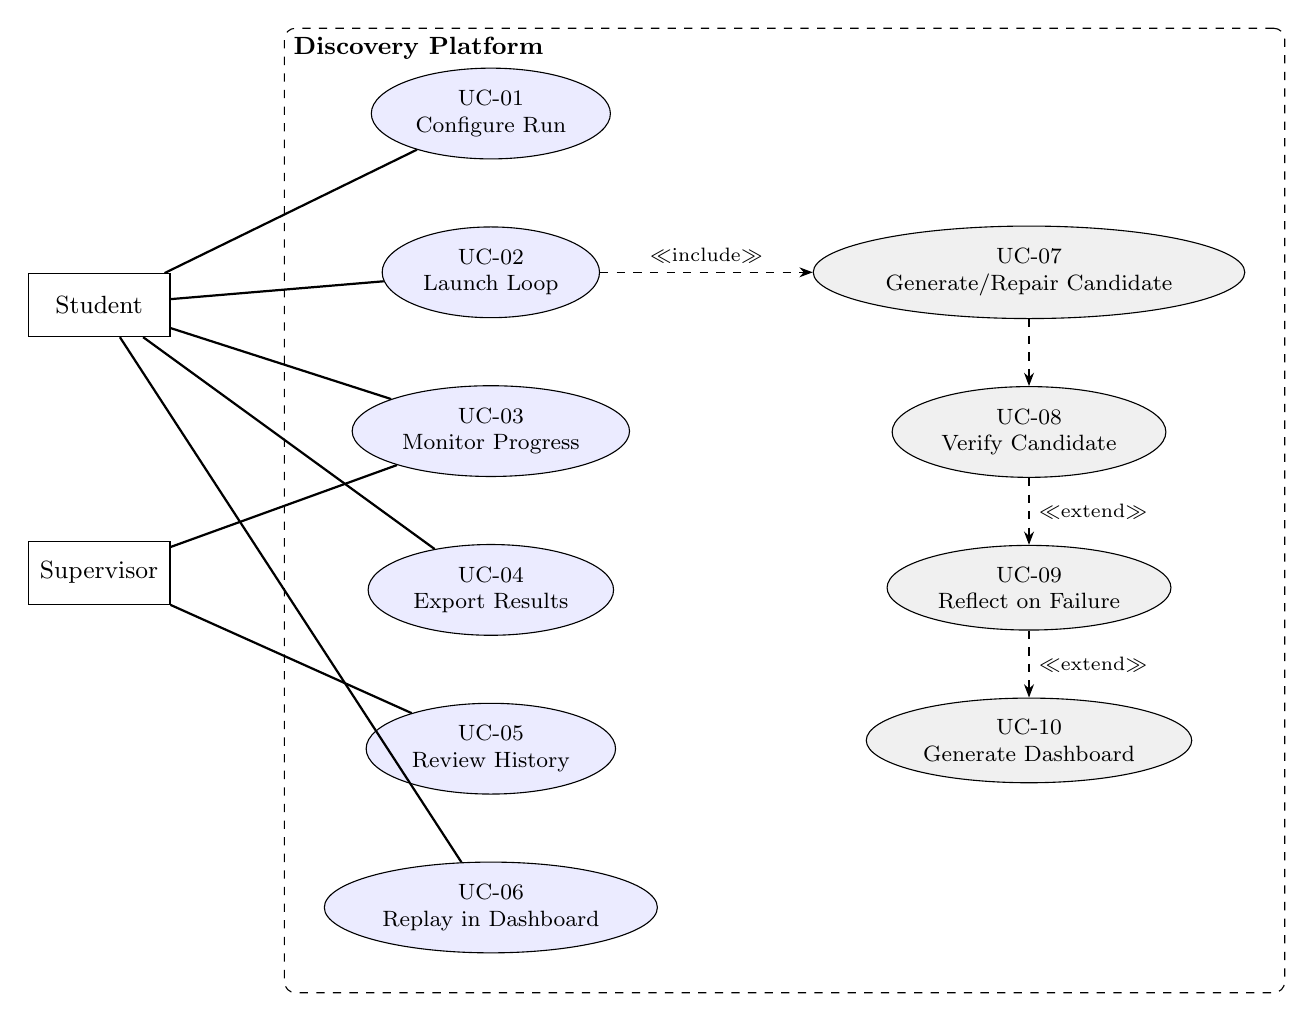
\begin{tikzpicture}[node distance=0.85cm]
\node[usecase] (config)  {UC-01\\Configure Run};
\node[usecase] (launch)  [below=of config]  {UC-02\\Launch Loop};
\node[usecase] (monitor) [below=of launch]   {UC-03\\Monitor Progress};
\node[usecase] (export)  [below=of monitor]  {UC-04\\Export Results};
\node[usecase] (review)  [below=of export]   {UC-05\\Review History};
\node[usecase] (replay)  [below=of review]   {UC-06\\Replay in Dashboard};
\node[internal] (gen)     [right=2.7cm of launch]  {UC-07\\Generate/Repair Candidate};
\node[internal] (verify)  [below=of gen]           {UC-08\\Verify Candidate};
\node[internal] (reflect) [below=of verify]        {UC-09\\Reflect on Failure};
\node[internal] (dash)    [below=of reflect]       {UC-10\\Generate Dashboard};
\begin{scope}[on background layer]
\node[boundary, fit=(config)(launch)(monitor)(export)(review)(replay)(gen)(verify)(reflect)(dash)] (bound) {};
\end{scope}
\node[anchor=north west, font=\small\bfseries] at (bound.north west) {Discovery Platform};
\node[actor] (student)    [left=2.3cm of monitor, yshift=1.6cm] {Student};
\node[actor] (supervisor) [left=2.3cm of monitor, yshift=-1.8cm] {Supervisor};
\draw[link] (student) -- (config);
\draw[link] (student) -- (launch);
\draw[link] (student) -- (monitor);
\draw[link] (student) -- (export);
\draw[link] (student) -- (replay);
\draw[link] (supervisor) -- (monitor);
\draw[link] (supervisor) -- (review);
\draw[inc] (launch) -- node[above, font=\scriptsize] {$\ll$include$\gg$} (gen);
\draw[inc] (gen) -- (verify);
\draw[inc] (verify) -- node[right, font=\scriptsize] {$\ll$extend$\gg$} (reflect);
\draw[inc] (reflect) -- node[right, font=\scriptsize] {$\ll$extend$\gg$} (dash);
\end{tikzpicture}
\caption{Use case diagram. White ellipses are user-triggered; grey ellipses are performed automatically by the system inside the evolutionary loop.}
\label{fig:uc}
\end{figure}

\begin{center}
\footnotesize
\setlength{\tabcolsep}{4pt}
\renewcommand{\arraystretch}{1.2}
\newcolumntype{R}[1]{>{\raggedright\arraybackslash}p{#1}}
\begin{longtable}{|R{0.8cm}|R{2.6cm}|R{2.4cm}|R{2.4cm}|R{3.2cm}|}
\toprule
\textbf{ID} & \textbf{Function} & \textbf{Given} & \textbf{When} & \textbf{Then} \\
\midrule
\endfirsthead
\toprule
\textbf{ID} & \textbf{Function} & \textbf{Given} & \textbf{When} & \textbf{Then} \\
\midrule
\endhead
\bottomrule
\endfoot

US-01 & configure\_run & I am a student & I set the problem, provider, and evolutionary parameters & The configuration is validated and saved \\
\addlinespace[1pt]
US-02 & launch\_run & A run is configured & I launch it & The system evolves and tests candidates until a stop condition \\
\addlinespace[1pt]
US-03 & monitor\_progress & A run is active or finished & I query its status & I see generation, best fitness, and failure patterns \\
\addlinespace[1pt]
US-04 & export\_results & A run has produced results & I export it & A readable report and a structured data file are written \\
\addlinespace[1pt]
US-05 & review\_history & Previous runs exist & I select one & I see its summary and can drill into generations \\
\addlinespace[1pt]
US-06 & replay\_dashboard & A run has dashboards & I open the latest dashboard & I replay the generation history on the timeline \\
\addlinespace[1pt]
US-07 & generate\_candidate & A parent and prompt are ready & The loop needs offspring & A new candidate is written to disk \\
\addlinespace[1pt]
US-08 & verify\_candidate & A candidate exists & The loop verifies it & Its invariant is checked over operation sequences; it is marked correct or incorrect, with efficiency and failing cases recorded \\
\addlinespace[1pt]
US-09 & reflect\_failure & A candidate failed & The loop requests a reflection & A structured reflection and repair hints are produced for the next generation \\
\addlinespace[1pt]
US-10 & generate\_dashboard & A generation completes & Every $N$ generations or at run end & A self-contained HTML dashboard is written \\
\caption{User stories in given-when-then form.}
\label{tab:us}
\end{longtable}
\end{center}

% ============================================================
\section{Functional Requirements}

Requirements are unique, atomic, and testable. Each states input, precondition, behavior, output, error or rejection behavior, and priority (Must, Should, Could). The ID prefix names the capability: \texttt{FR-CMD} (CLI), \texttt{FR-UI} (dashboard), \texttt{FR-VER} (verification), \texttt{FR-AGENT} (agents and provider), \texttt{FR-EVO} (evolutionary loop), \texttt{FR-PER} (persistence and recovery).

\subsection{CLI and Run Control}

\begin{longtable}{@{}p{2.2cm}p{10.6cm}@{}}
\toprule
\textbf{ID} & \textbf{Requirement} \\
\midrule
\endfirsthead
\toprule
\textbf{ID} & \textbf{Requirement} \\
\midrule
\endhead
\bottomrule
\endfoot

\texttt{FR-CMD-01} & \textbf{Configure run.} Input: a YAML configuration file (Section~\ref{sec:interfaces}). Precondition: none. Behavior: parse and validate the configuration; resolve the run ID; write the run manifest. Output: a valid configuration stored under the run directory. Error: on any invalid field, reject with a named-field message and exit non-zero; do not start a run. Priority: Must. \\
\addlinespace[2pt]

\texttt{FR-CMD-02} & \textbf{Launch run.} Input: a validated configuration. Precondition: \texttt{FR-CMD-01} succeeded and the provider is reachable. Behavior: initialize the population, then run the evolutionary loop (Section~\ref{sec:evo}) until a stop condition. Output: terminal progress lines and per-generation artifacts. Error: if the provider is unreachable at launch, abort with a clear message and exit non-zero. Priority: Must. \\
\addlinespace[2pt]

\texttt{FR-CMD-03} & \textbf{Monitor progress.} Input: a run ID. Precondition: the run exists. Behavior: read the latest checkpoint and report generation, best fitness, pass rate, and recent failures. Output: a status summary to the terminal. Error: if the run ID is unknown, report it and exit non-zero. Priority: Must. \\
\addlinespace[2pt]

\texttt{FR-CMD-04} & \textbf{Export results.} Input: a run ID. Precondition: the run has at least one completed generation. Behavior: write a human-readable report and a machine-readable results file. Output: \texttt{run\_summary.json} and a report file. Error: if no results exist, report it and exit non-zero. Priority: Must. \\
\addlinespace[2pt]

\texttt{FR-CMD-05} & \textbf{Review history.} Input: none, or a run ID filter. Precondition: at least one prior run exists. Behavior: list runs with their summaries (problem, generations, best fitness, outcome). Output: a history listing. Error: if no runs exist, state that and exit zero. Priority: Should. \\
\addlinespace[2pt]

\texttt{FR-CMD-06} & \textbf{Steer between runs.} Input: an edited configuration file. Precondition: a prior run exists. Behavior: start a new run from the edited configuration, optionally seeding the population from a prior run's best candidate. Output: a new run ID and progress. Error: an invalid edit is rejected as in \texttt{FR-CMD-01}. Priority: Should. \\
\addlinespace[2pt]

\texttt{FR-CMD-07} & \textbf{Pause and resume.} Input: a run ID. Precondition: the run was checkpointed. Behavior: pause stops the loop after the current generation; resume continues from the latest checkpoint. Output: the run continues from the saved generation. Error: if the checkpoint is corrupt, refuse to resume and report it (see \texttt{SC-10}). Priority: Should. \\
\bottomrule
\end{longtable}

\subsection{Dashboard}

\begin{longtable}{@{}p{2.2cm}p{10.6cm}@{}}
\toprule
\textbf{ID} & \textbf{Requirement} \\
\midrule
\endfirsthead
\toprule
\textbf{ID} & \textbf{Requirement} \\
\midrule
\endhead
\bottomrule
\endfoot

\texttt{FR-UI-01} & \textbf{Generate dashboard.} Input: run artifacts. Precondition: a generation has completed. Behavior: render a self-contained static HTML dashboard (all CSS and JavaScript inline, no external fetches). Output: a dashboard file written to the run directory. Error: on render failure, log it and continue the run; the dashboard is not a stop condition. Priority: Must. \\
\addlinespace[2pt]

\texttt{FR-UI-02} & \textbf{Generation-history replay.} Input: the dashboard. Precondition: at least two generations exist. Behavior: a client-side slider steps through generations, updating the displayed population and fitness. Output: the replay reflects each generation's state. Error: if the data is incomplete, the slider stops at the last complete generation. Priority: Must. \\
\addlinespace[2pt]

\texttt{FR-UI-03} & \textbf{Charts.} Input: the dashboard. Precondition: metrics exist. Behavior: show fitness-over-generation and work-ratio-over-generation charts. Output: rendered charts. Error: if a metric is absent, omit that chart and note it. Priority: Should. \\
\addlinespace[2pt]

\texttt{FR-UI-04} & \textbf{Failure list.} Input: the dashboard. Precondition: at least one failure exists. Behavior: list failing candidates with their failing case (graph, operation, invariant violated). Output: a navigable failure list. Error: if there are no failures, show an empty state. Priority: Must. \\
\addlinespace[2pt]

\texttt{FR-UI-05} & \textbf{Configuration view.} Input: the dashboard. Precondition: a run manifest exists. Behavior: display the run's configuration and the steering instructions (how to edit the config between runs). Output: a configuration panel. Error: if the manifest is missing, show a placeholder. Priority: Should. \\
\addlinespace[2pt]

\texttt{FR-UI-06} & \textbf{Dashboard cadence.} Input: the configuration field \texttt{dashboard\_every}. Precondition: the run is active. Behavior: generate a dashboard every $N$ generations (default $N=10$) and always at run end. Output: dashboards at the configured cadence. Error: an invalid $N$ is rejected at configuration time. Priority: Must. \\
\bottomrule
\end{longtable}

\subsection{Verification Engine}

\begin{longtable}{@{}p{2.2cm}p{10.6cm}@{}}
\toprule
\textbf{ID} & \textbf{Requirement} \\
\midrule
\endfirsthead
\toprule
\textbf{ID} & \textbf{Requirement} \\
\midrule
\endhead
\bottomrule
\endfoot

\texttt{FR-VER-01} & \textbf{Exhaustive enumeration.} Input: a vertex size $n$ with $n \le 5$. Precondition: \texttt{nauty} is available. Behavior: enumerate all non-isomorphic digraphs on $n$ vertices via \texttt{geng} and \texttt{directg}, converting each to the adjacency-matrix representation. Output: a cached set of base graphs per $n$. Error: if \texttt{nauty} is missing or fails, abort the run with a clear message. Priority: Must. \\
\addlinespace[2pt]

\texttt{FR-VER-02} & \textbf{Random sampling.} Input: a vertex size $n > 5$ and a sampling budget. Precondition: none. Behavior: sample random graphs and operation sequences up to the configured budget. Output: a sampled test set. Error: if the budget is invalid, reject at configuration time. Priority: Must. \\
\addlinespace[2pt]

\texttt{FR-VER-03} & \textbf{Operation sequences.} Input: a base graph. Precondition: the graph size is valid. Behavior: generate sequences of interleaved edge insertions and deletions, each at most \texttt{max\_ops\_per\_sequence} operations (default 10). Output: a set of operation sequences. Error: an operation on a nonexistent or already-present edge is rejected as an invalid graph operation (see \texttt{SC-08}). Priority: Must. \\
\addlinespace[2pt]

\texttt{FR-VER-04} & \textbf{Invariant checking.} Input: a candidate output after each operation. Precondition: the problem's invariant is defined. Behavior: check the invariant after every operation in the sequence; record the first violation. Output: pass/fail per sequence with the violating operation. Error: a candidate that crashes or times out is recorded as \texttt{CRASH}, not as a pass. Priority: Must. \\
\addlinespace[2pt]

\texttt{FR-VER-05} & \textbf{Fitness scoring.} Input: per-sequence pass/fail results. Precondition: the candidate was executed. Behavior: set fitness to the fraction of sequences whose invariant held throughout. Output: a fitness value in $[0,1]$. Error: if no sequence could be executed, fitness is 0. Priority: Must. \\
\addlinespace[2pt]

\texttt{FR-VER-06} & \textbf{Efficiency scoring.} Input: candidate work and offline-recomputation work. Precondition: the candidate ran to completion on the sequence. Behavior: compute \texttt{work\_ratio} as candidate work divided by offline-recomputation work, where work counts vertices visited and edges scanned per update. Output: a \texttt{work\_ratio} value. Error: if the candidate did not complete, no efficiency is recorded. Priority: Must. \\
\addlinespace[2pt]

\texttt{FR-VER-07} & \textbf{Efficiency acceptance.} Input: a \texttt{work\_ratio}. Precondition: the candidate is correct (fitness 1.0). Behavior: mark the candidate an efficiency improvement only if \texttt{work\_ratio} $< 1$. Output: an efficiency-improvement flag. Error: a \texttt{work\_ratio} $\ge 1$ means no improvement; it is not an error. Priority: Must. \\
\addlinespace[2pt]

\texttt{FR-VER-08} & \textbf{Verifier self-test.} Input: a known-good reference algorithm and a known-bad mutation. Precondition: the verifier is built. Behavior: run both through the full verification path before any experiment. Output: the known-good is accepted and the known-bad is rejected. Error: if the known-good is rejected or the known-bad is accepted, the verifier is faulty and no experiment may run. Priority: Must. \\
\addlinespace[2pt]

\texttt{FR-VER-09} & \textbf{Trust boundary.} Input: none. Precondition: none. Behavior: the verification engine is pre-built and is not readable or writable by any agent; agents receive only fitness and structured failure summaries, never the test code. Output: enforced isolation. Error: N/A (enforced by construction). Priority: Must. \\
\bottomrule
\end{longtable}

\subsection{Agents and Model Provider}

\begin{longtable}{@{}p{2.2cm}p{10.6cm}@{}}
\toprule
\textbf{ID} & \textbf{Requirement} \\
\midrule
\endfirsthead
\toprule
\textbf{ID} & \textbf{Requirement} \\
\midrule
\endhead
\bottomrule
\endfoot

\texttt{FR-AGENT-01} & \textbf{Provider abstraction.} Input: a provider name and model. Precondition: the provider is configured. Behavior: all model calls go through a single vendor-agnostic interface; no component depends on a specific vendor. Output: model responses. Error: an unknown provider is rejected at configuration time. Priority: Must. \\
\addlinespace[2pt]

\texttt{FR-AGENT-02} & \textbf{Generation role.} Input: a problem definition and a parent candidate. Precondition: the provider is reachable. Behavior: produce a new candidate implementing the candidate interface. Output: a candidate Python file. Error: on a malformed response, retry per \texttt{NFR-REL-02}; after exhaustion, record the candidate as failed. Priority: Must. \\
\addlinespace[2pt]

\texttt{FR-AGENT-03} & \textbf{Repair role.} Input: a failed candidate and its reflection. Precondition: a reflection exists. Behavior: produce a repaired candidate. Output: a repaired Python file. Error: as in \texttt{FR-AGENT-02}. Priority: Must. \\
\addlinespace[2pt]

\texttt{FR-AGENT-04} & \textbf{Reflection role.} Input: a failing case (graph, operation sequence, violated invariant, expected vs actual). Precondition: a candidate failed. Behavior: produce a structured reflection with failure description, root cause, and repair hints. Output: a reflection file. Error: if reflection fails after retries, proceed without it (diversity may still recover). Priority: Must. \\
\addlinespace[2pt]

\texttt{FR-AGENT-05} & \textbf{Prompt logging.} Input: every model call. Precondition: none. Behavior: log the full prompt and response used for each call, keyed by run and candidate. Output: prompt logs under the run directory. Error: N/A. Priority: Should. \\
\addlinespace[2pt]

\texttt{FR-AGENT-06} & \textbf{Plateau specialization (experiment).} Input: a plateau signal (no fitness gain for $k$ generations). Precondition: the experiment flag is set. Behavior: optionally spawn a specialized agent targeting the stalled failure pattern. Output: an additional agent and its candidates. Error: if not enabled, the loop continues with the fixed roles. Priority: Could. \\
\addlinespace[2pt]

\texttt{FR-AGENT-07} & \textbf{Lean formalization role.} Input: a candidate that passed bounded verification and its problem definition/invariant. Precondition: the candidate is empirically validated. Behavior: produce an honest Lean~4 proof that the candidate maintains its invariant under every update, in the \texttt{thesis-lean} project, with no \texttt{axiom}/\texttt{sorry}/\texttt{unsafe}. Output: one or more \texttt{.lean} modules and a successful \texttt{lake build}. Error: if a lemma resists proof, report the gap explicitly rather than introducing \texttt{sorry}. Priority: Must (final phase). \\
\bottomrule
\end{longtable}

\subsection{Evolutionary Loop}
\label{sec:evo}

\begin{longtable}{@{}p{2.2cm}p{10.6cm}@{}}
\toprule
\textbf{ID} & \textbf{Requirement} \\
\midrule
\endfirsthead
\toprule
\textbf{ID} & \textbf{Requirement} \\
\midrule
\endhead
\bottomrule
\endfoot

\texttt{FR-EVO-01} & \textbf{Elitism.} Input: the scored population. Precondition: a generation completed. Behavior: keep the top-k candidates by fitness into the next generation. Output: the surviving population. Error: if fewer than k candidates exist, keep all. Priority: Must. \\
\addlinespace[2pt]

\texttt{FR-EVO-02} & \textbf{Repair of failures.} Input: failed candidates with reflections. Precondition: a reflection exists. Behavior: repair failed candidates via the repair role rather than discarding them. Output: repaired candidates in the next population. Error: if repair is unavailable, the candidate is discarded. Priority: Must. \\
\addlinespace[2pt]

\texttt{FR-EVO-03} & \textbf{Diversity.} Input: the population. Precondition: the population has converged (low diversity). Behavior: introduce random mutation to maintain exploration. Output: mutated candidates. Error: N/A. Priority: Must. \\
\addlinespace[2pt]

\texttt{FR-EVO-04} & \textbf{Stop on success.} Input: the scored population. Precondition: a generation completed. Behavior: stop the loop when any candidate reaches fitness 1.0. Output: the run ends with the successful candidate. Error: N/A. Priority: Must. \\
\addlinespace[2pt]

\texttt{FR-EVO-05} & \textbf{Stop on max generations.} Input: the generation counter. Precondition: none. Behavior: stop when the generation count reaches \texttt{max\_generations}. Output: the run ends with the best candidate found. Error: N/A. Priority: Must. \\
\addlinespace[2pt]

\texttt{FR-EVO-06} & \textbf{All-failed generation.} Input: a generation in which every candidate failed. Precondition: the loop is active. Behavior: log a warning, apply diversity, and continue to the next generation. Output: the loop continues. Error: if $m$ consecutive all-failed generations occur, stop and report. Priority: Should. \\
\bottomrule
\end{longtable}

\subsection{Persistence and Recovery}

\begin{longtable}{@{}p{2.2cm}p{10.6cm}@{}}
\toprule
\textbf{ID} & \textbf{Requirement} \\
\midrule
\endfirsthead
\toprule
\textbf{ID} & \textbf{Requirement} \\
\midrule
\endhead
\bottomrule
\endfoot

\texttt{FR-PER-01} & \textbf{Per-generation artifacts.} Input: a completed generation. Precondition: none. Behavior: write a JSON state file, the candidate Python files, reflections, and per-candidate results. Output: artifacts under the run directory (Section~\ref{sec:interfaces}). Error: on write failure, mark the checkpoint incomplete and report it. Priority: Must. \\
\addlinespace[2pt]

\texttt{FR-PER-02} & \textbf{Atomic writes.} Input: any artifact. Precondition: none. Behavior: write to a temporary file and rename into place so a crash never leaves a half-written artifact. Output: a complete artifact or the previous one. Error: a torn write is impossible by construction. Priority: Must. \\
\addlinespace[2pt]

\texttt{FR-PER-03} & \textbf{Checkpoint and resume.} Input: a run ID. Precondition: at least one checkpoint exists. Behavior: checkpoint every generation; on resume, reload the latest complete checkpoint and continue. Output: the run resumes from the saved generation. Error: on a corrupt checkpoint, refuse to resume and report the last good generation (see \texttt{SC-10}). Priority: Must. \\
\bottomrule
\end{longtable}

% ============================================================
\section{Detailed Scenarios}
\label{sec:scenarios}

Each scenario names the actor, precondition, trigger, main flow, outcome, and the alternate, error, boundary, permission, and failure behaviors. These expand the use cases in Section~\ref{sec:usecases}.

\subsubsection{SC-01: Launch a run}

\begin{description}[style=nextline, leftmargin=2.4cm]
  \item[Actor / precondition] Student; a validated configuration exists.
  \item[Trigger] The student runs the launch command.
  \item[Main flow] The system initializes the population, enters the evolutionary loop, and prints a progress line each generation.
  \item[Outcome] The run proceeds to a stop condition.
  \item[Alternate] If the student wants to seed from a prior run, the launch accepts a seed run ID.
  \item[Error / failure] If the provider is unreachable, the launch aborts with a clear message and non-zero exit; no partial run is started.
  \item[Boundary] A population size of 1 is allowed (degenerate but valid).
  \item[Permission] Only the student launches runs; the supervisor does not.
\end{description}

\subsubsection{SC-02: Pause and resume}

\begin{description}[style=nextline, leftmargin=2.4cm]
  \item[Actor / precondition] Student; the run is active and has at least one checkpoint.
  \item[Trigger] The student pauses, then later resumes.
  \item[Main flow] Pause stops the loop after the current generation; resume reloads the latest checkpoint and continues.
  \item[Outcome] The run continues from the saved generation without re-doing completed work.
  \item[Alternate] The student may resume on a different machine from the same run directory.
  \item[Error / failure] If the latest checkpoint is corrupt, resume is refused and the last good generation is reported (SC-10).
  \item[Boundary] Pausing with zero completed generations is a no-op.
  \item[Permission] The student controls pause/resume; the supervisor is read-only.
\end{description}

\subsubsection{SC-03: Replay generation history in the dashboard}

\begin{description}[style=nextline, leftmargin=2.4cm]
  \item[Actor / precondition] Student or supervisor; the run produced at least two generations and a dashboard.
  \item[Trigger] The user opens the latest dashboard and moves the replay slider.
  \item[Main flow] The client-side JavaScript steps through generations, updating the population table and fitness chart.
  \item[Outcome] The user sees the full history of the run in the browser, offline.
  \item[Alternate] The user jumps directly to a generation by number.
  \item[Error / failure] If a generation's data is incomplete, the slider stops at the last complete generation and notes the gap.
  \item[Boundary] A single-generation run shows a static dashboard with no replay motion.
  \item[Permission] Both actors may view and replay.
\end{description}

\subsubsection{SC-04: Agent plateau}

\begin{description}[style=nextline, leftmargin=2.4cm]
  \item[Actor / precondition] System (automatic); fitness has not improved for $k$ generations.
  \item[Trigger] The plateau detector fires.
  \item[Main flow] The loop applies diversity (random mutation). If the plateau-specialization experiment is enabled, a specialized agent is spawned for the stalled failure pattern.
  \item[Outcome] Exploration resumes; fitness may recover.
  \item[Alternate] If specialization is disabled, only diversity is applied.
  \item[Error / failure] If the specialized agent produces no valid candidate, it is retired and the fixed roles continue.
  \item[Boundary] A plateau of one generation does not trigger action.
  \item[Permission] No human action is required; this is automatic.
\end{description}

\subsubsection{SC-05: LLM API failure and retry exhaustion}

\begin{description}[style=nextline, leftmargin=2.4cm]
  \item[Actor / precondition] System (automatic); a model call is in flight.
  \item[Trigger] The provider returns an error or times out.
  \item[Main flow] The call is retried up to 3 times with exponential backoff (NFR-REL-02).
  \item[Outcome] A successful retry proceeds normally.
  \item[Alternate] A different model on the same provider may be tried if configured.
  \item[Error / failure] After 3 failed attempts, the candidate is recorded as failed and the loop continues with the next candidate.
  \item[Boundary] A single transient failure does not stop the run.
  \item[Permission] No human action; the run degrades gracefully.
\end{description}

\subsubsection{SC-06: Candidate timeout}

\begin{description}[style=nextline, leftmargin=2.4cm]
  \item[Actor / precondition] System (automatic); a candidate is executing in the sandbox.
  \item[Trigger] The candidate exceeds the per-candidate timeout (default 30 s).
  \item[Main flow] The sandbox kills the process; the candidate is recorded as \texttt{CRASH} with a timeout flag.
  \item[Outcome] The loop continues with the next candidate.
  \item[Alternate] The timeout is configurable per run.
  \item[Error / failure] A timeout is a failure, not a pass; it never halts the run.
  \item[Boundary] A candidate that finishes exactly at the limit is treated as a timeout.
  \item[Permission] No human action required.
\end{description}

\subsubsection{SC-07: Verifier disagreement}

\begin{description}[style=nextline, leftmargin=2.4cm]
  \item[Actor / precondition] System (automatic); a candidate's invariant result is unexpected.
  \item[Trigger] A candidate that should be correct fails, or a clearly wrong candidate passes.
  \item[Main flow] The system flags the disagreement and records the case; the verifier self-test (FR-VER-08) is re-run.
  \item[Outcome] If the self-test fails, the run is halted and the verifier is treated as faulty.
  \item[Alternate] If the self-test passes, the case is logged as a genuine candidate failure.
  \item[Error / failure] A faulty verifier must not be used to score experiments.
  \item[Boundary] Disagreement on a single sequence is logged, not fatal, unless the self-test fails.
  \item[Permission] The supervisor is notified of any verifier fault.
\end{description}

\subsubsection{SC-08: Invalid graph operation}

\begin{description}[style=nextline, leftmargin=2.4cm]
  \item[Actor / precondition] System (automatic); an operation sequence is being built.
  \item[Trigger] A generated operation would insert an edge already present or delete an edge absent.
  \item[Main flow] The operation is rejected and replaced with a valid one; the sequence stays within bounds.
  \item[Outcome] Only valid operation sequences reach the candidate.
  \item[Alternate] If a candidate itself reports an invalid operation, it is recorded as a candidate fault.
  \item[Error / failure] Rejection is silent to the candidate; it is logged to the run.
  \item[Boundary] An operation on a vertex outside the graph size is invalid.
  \item[Permission] No human action required.
\end{description}

\subsubsection{SC-09: All candidates failed in a generation}

\begin{description}[style=nextline, leftmargin=2.4cm]
  \item[Actor / precondition] System (automatic); a generation produced no passing candidate.
  \item[Trigger] Every candidate in the generation failed or crashed.
  \item[Main flow] The loop logs a warning, applies diversity, and continues to the next generation.
  \item[Outcome] The run continues; recovery is expected via diversity.
  \item[Alternate] If $m$ consecutive generations are all-failed, the run stops and reports.
  \item[Error / failure] A single all-failed generation is not fatal.
  \item[Boundary] $m$ is configurable (default 5).
  \item[Permission] The student is informed via the terminal and dashboard.
\end{description}

\subsubsection{SC-10: Checkpoint corruption}

\begin{description}[style=nextline, leftmargin=2.4cm]
  \item[Actor / precondition] Student; a resume is requested.
  \item[Trigger] The latest checkpoint fails validation (bad JSON or missing fields).
  \item[Main flow] The system refuses to resume from the corrupt checkpoint and scans for the last complete checkpoint.
  \item[Outcome] The run resumes from the last good checkpoint, or reports that no good checkpoint exists.
  \item[Alternate] The student may start a fresh run from the configuration.
  \item[Error / failure] Atomic writes (FR-PER-02) make corruption rare; a corrupt state is never silently accepted.
  \item[Boundary] If all checkpoints are corrupt, resume is impossible and a fresh run is required.
  \item[Permission] The student decides whether to resume or restart.
\end{description}

% ============================================================
\section{Acceptance Criteria}

Every complex contribution and high-priority requirement has observable acceptance criteria naming the demonstration, test, output, or artifact and the threshold. Subjective terms are avoided.

\begin{center}
\footnotesize
\setlength{\tabcolsep}{4pt}
\renewcommand{\arraystretch}{1.2}
\begin{longtable}{@{}p{2.6cm}p{6.4cm}p{4.2cm}@{}}
\toprule
\textbf{ID} & \textbf{Acceptance criterion} & \textbf{Evidence / threshold} \\
\midrule
\endfirsthead
\toprule
\textbf{ID} & \textbf{Acceptance criterion} & \textbf{Evidence / threshold} \\
\midrule
\endhead
\bottomrule
\endfoot

AC-01 & The UI framework launches, monitors, and replays a multi-generation run end to end. & A recorded demo: CLI launch, terminal progress, and dashboard replay of at least 10 generations with no error. \\
\addlinespace[2pt]
AC-02 & The verification engine accepts a known-good algorithm. & The verifier self-test (FR-VER-08) reports the known-good candidate accepted on $n \le 5$. \\
\addlinespace[2pt]
AC-03 & The verification engine rejects a known-bad mutation. & The self-test reports the known-bad candidate rejected, with the violating operation recorded. \\
\addlinespace[2pt]
AC-04 & Zero false negatives on $n \le 5$. & Across all non-isomorphic digraphs for $n=1$ to $5$, every known-correct algorithm passes; the false-negative count is 0. \\
\addlinespace[2pt]
AC-05 & A correct dynamic BFS is discovered within bounded generations. & An unattended run reaches fitness 1.0 for dynamic BFS within the configured \texttt{max\_generations}, with no human intervention. \\
\addlinespace[2pt]
AC-06 & Efficiency improvement is measured correctly. & A correct candidate is flagged as an efficiency improvement if and only if \texttt{work\_ratio} $< 1$. \\
\addlinespace[2pt]
AC-07 & A run survives interruption. & A run paused or killed mid-generation resumes from the latest checkpoint and completes without losing completed generations. \\
\addlinespace[2pt]
AC-08 & Candidate code is isolated. & A candidate that attempts network access or writes outside its sandbox is blocked; the run continues. \\
\addlinespace[2pt]
AC-09 & Results are reproducible. & Two runs with the same configuration and fixed seeds produce identical fitness trajectories and the same best candidate. \\
\bottomrule
\caption{Acceptance criteria with named evidence and thresholds.}
\label{tab:acceptance}
\end{longtable}
\end{center}

% ============================================================
\section{Data Model and Business Rules}
\label{sec:srsdata}

\subsection{Entities}

\begin{center}
\footnotesize
\setlength{\tabcolsep}{4pt}
\begin{longtable}{@{}p{2.6cm}p{4.6cm}p{5.6cm}@{}}
\toprule
\textbf{Entity} & \textbf{Key attributes} & \textbf{Notes} \\
\midrule
\endfirsthead
\toprule
\textbf{Entity} & \textbf{Key attributes} & \textbf{Notes} \\
\midrule
\endhead
\bottomrule
\endfoot

Run & run ID, problem, config, start/end time, outcome & Top-level container; owns all other entities. \\
\addlinespace[2pt]
Generation & run ID, generation number, timestamp, best fitness & One round of the loop; checkpointed. \\
\addlinespace[2pt]
Candidate & candidate ID, code path, fitness, work ratio, state, parent ID & An algorithm attempt; state in \{NEW, TESTING, PASS, FAIL, CRASH, DISCARDED\}. \\
\addlinespace[2pt]
Parent & candidate ID of the parent & Lineage link for elitism and repair. \\
\addlinespace[2pt]
Reflection & candidate ID, failure description, root cause, repair hints & Produced by the reflector role. \\
\addlinespace[2pt]
Failure & candidate ID, graph, operation, invariant violated & A single failing case. \\
\addlinespace[2pt]
Metric & candidate ID, tests passed, tests total, work ratio, timing & Per-candidate measurement. \\
\bottomrule
\caption{Data entities.}
\label{tab:entities}
\end{longtable}
\end{center}

\subsection{Validation and uniqueness}

\begin{itemize}
  \item Run IDs and candidate IDs are unique within the run directory; candidate IDs encode generation and index (for example \texttt{gen042\_c03}).
  \item Configuration fields are validated at launch: population size 1 to 50, max generations 1 to 1000, timeout 1 to 300 seconds, graph size at least 1, \texttt{dashboard\_every} at least 1.
  \item Candidate code must parse as valid Python before execution; a syntax error is recorded as \texttt{CRASH}.
  \item Operation sequences contain only valid edge operations (SC-08).
\end{itemize}

\subsection{Lifecycle and ownership}

\begin{itemize}
  \item A candidate moves NEW to TESTING to one of PASS, FAIL, or CRASH, then to DISCARDED if removed from the population.
  \item The orchestrator owns the run and generation state; the verifier owns per-candidate results; the agents own candidate code and reflections.
  \item The trusted verifier is owned by the student as pre-built infrastructure and is not modifiable by agents (FR-VER-09).
\end{itemize}

\subsection{Retention and crash-safe persistence}

\begin{itemize}
  \item All artifacts are retained per run under the run directory; nothing is auto-deleted.
  \item Every write is atomic (write to temporary file, then rename), so a crash leaves either the old or the new complete artifact, never a torn one (FR-PER-02).
  \item A checkpoint is written every generation (FR-PER-03), enabling resume after interruption.
\end{itemize}

% ============================================================
\section{Interfaces, File Formats, and Roles}
\label{sec:interfaces}

\subsection{CLI command schema}

\begin{center}
\footnotesize
\setlength{\tabcolsep}{4pt}
\begin{longtable}{@{}p{4.2cm}p{8.6cm}@{}}
\toprule
\textbf{Command} & \textbf{Description and failure behavior} \\
\midrule
\endfirsthead
\toprule
\textbf{Command} & \textbf{Description and failure behavior} \\
\midrule
\endhead
\bottomrule
\endfoot

\texttt{run configure <config.yaml>} & Validate and store the configuration; exit non-zero on an invalid field. \\
\addlinespace[2pt]
\texttt{run start <config.yaml>} & Launch the evolutionary loop; exit non-zero if the provider is unreachable. \\
\addlinespace[2pt]
\texttt{run status <run\_id>} & Report generation, best fitness, pass rate, recent failures; exit non-zero on unknown run. \\
\addlinespace[2pt]
\texttt{run export <run\_id>} & Write the report and results file; exit non-zero if no results exist. \\
\addlinespace[2pt]
\texttt{run history} & List prior runs with summaries; exit zero if none. \\
\addlinespace[2pt]
\texttt{run resume <run\_id>} & Resume from the latest good checkpoint; refuse on a corrupt checkpoint. \\
\bottomrule
\caption{CLI commands.}
\label{tab:cli}
\end{longtable}
\end{center}

\subsection{YAML configuration format}

\begin{verbatim}
problem: dynamic_bfs          # dynamic_bfs | dynamic_dfs | dynamic_mcs | dynamic_scc | dynamic_lbfs
graph_mode: directed          # directed | undirected (undirected for dynamic_mcs)
model_provider: openai        # vendor-agnostic provider name
model: <model-id>
population_size: 10
max_generations: 100
max_ops_per_sequence: 10
graph_max_size: 5             # exhaustive for n <= 5
sampling_budget: 100          # random sequences for n > 5
timeout_seconds: 30
model_call_timeout_seconds: 60
llm_max_retries: 3
dashboard_every: 10
seed: 42
\end{verbatim}

\subsection{Model-provider interface}

The provider abstraction exposes three operations, one per agent role: \texttt{generate(problem, parent) -> code}, \texttt{repair(candidate, reflection) -> code}, and \texttt{reflect(failing\_case) -> reflection}. Each returns text and is subject to the per-call timeout and retry policy. The interface is vendor-agnostic; a new provider is added by implementing these three operations.

\subsection{Dashboard file format}

A dashboard is a single self-contained HTML file with inline CSS and JavaScript and no external resource fetches. It embeds the generation history as a JSON payload and renders the replay slider, charts, failure list, and configuration view client-side.

\subsection{Candidate, reflection, and result file formats}

\begin{itemize}
  \item \textbf{Candidate:} a self-contained Python file exposing \texttt{insert\_edge(graph, edge, state)} and \texttt{delete\_edge(graph, edge, state)}, where \texttt{graph} is the adjacency matrix of zeros and one and \texttt{state} is the algorithm's maintained structure.
  \item \textbf{Reflection:} a Markdown or JSON file with fields \texttt{failure\_description}, \texttt{root\_cause}, and \texttt{repair\_hints}.
  \item \textbf{Result:} \texttt{run\_summary.json} with per-generation statistics, the best candidate code path, efficiency metrics, and failure analysis.
\end{itemize}

\subsection{Run directory layout}

\begin{verbatim}
runs/<run_id>/
  manifest.json            # run ID, config, timestamps, outcome
  state/generation_001.json
  candidates/gen001_c01.py
  reflections/gen001_c01.md
  results/run_summary.json
  dashboards/dashboard_010.html
  prompts/                 # logged model calls
\end{verbatim}

\subsection{Role boundaries}

\begin{center}
\footnotesize
\setlength{\tabcolsep}{4pt}
\begin{longtable}{@{}p{3.2cm}p{4.6cm}p{5.0cm}@{}}
\toprule
\textbf{Component} & \textbf{Can read} & \textbf{Can write} \\
\midrule
\endfirsthead
\toprule
\textbf{Component} & \textbf{Can read} & \textbf{Can write} \\
\midrule
\endhead
\bottomrule
\endfoot

Orchestrator & run directory & run directory, sandbox \\
\addlinespace[2pt]
Agents (LLM) & prompts only & candidate and reflection files (via orchestrator) \\
\addlinespace[2pt]
Candidate code & its own sandbox & sandbox output only \\
\addlinespace[2pt]
Verifier & candidate outputs & results directory \\
\bottomrule
\caption{Read/write boundaries. Agents never read or write the verifier.}
\label{tab:roles}
\end{longtable}
\end{center}

% ============================================================
\section{Non-Functional Requirements}

Each quality attribute has a measurable target or evaluation method.

\begin{center}
\footnotesize
\setlength{\tabcolsep}{4pt}
\renewcommand{\arraystretch}{1.2}
\begin{longtable}{@{}p{2.4cm}p{2.0cm}p{8.4cm}@{}}
\toprule
\textbf{ID} & \textbf{Category} & \textbf{Requirement and target} \\
\midrule
\endfirsthead
\toprule
\textbf{ID} & \textbf{Category} & \textbf{Requirement and target} \\
\midrule
\endhead
\bottomrule
\endfoot

\texttt{NFR-PERF-01} & Performance & Exhaustive verification completes for all non-isomorphic digraphs up to $n \le 5$; the enumeration is cached so it runs once per size. \\
\addlinespace[2pt]
\texttt{NFR-PERF-02} & Performance & Operation sequences are bounded to at most 10 operations; the sampling budget for $n > 5$ is at most 100 sequences by default. \\
\addlinespace[2pt]
\texttt{NFR-PERF-03} & Performance & Per-candidate execution timeout defaults to 30 seconds; per-model-call timeout defaults to 60 seconds. \\
\addlinespace[2pt]
\texttt{NFR-PERF-04} & Performance & The dashboard renders a 10-generation run in under 5 seconds on a standard laptop (measured by timing the file render). \\
\addlinespace[2pt]
\texttt{NFR-REL-01} & Reliability & A checkpoint is written every generation; a run resumes from the latest good checkpoint after interruption (AC-07). \\
\addlinespace[2pt]
\texttt{NFR-REL-02} & Reliability & Transient model-call failures are retried up to 3 times with exponential backoff before a candidate is abandoned. \\
\addlinespace[2pt]
\texttt{NFR-SEC-01} & Security & Candidate code runs in real OS isolation (namespace or container), with no network access, a restricted filesystem, and CPU and memory limits. \\
\addlinespace[2pt]
\texttt{NFR-SEC-02} & Security & API keys are read from environment variables only and never written to code, configuration, or logs. \\
\addlinespace[2pt]
\texttt{NFR-PORT-01} & Portability & The tool runs on Python 3.11 or later with the \texttt{nauty} CLI and any configured LLM provider; no vendor lock-in. \\
\addlinespace[2pt]
\texttt{NFR-USAB-01} & Usability & All operations are available from the CLI and the dashboard; the dashboard is self-contained and viewable offline. \\
\addlinespace[2pt]
\texttt{NFR-USAB-02} & Usability & The dashboard's replay slider responds to input within 200 milliseconds (measured client-side). \\
\addlinespace[2pt]
\texttt{NFR-REPR-01} & Reproducibility & Runs use a fixed seed; all model prompts and responses are logged; a run manifest records the exact configuration. \\
\addlinespace[2pt]
\texttt{NFR-REPR-02} & Reproducibility & Two runs with identical configuration and seed produce identical fitness trajectories (AC-09). \\
\bottomrule
\caption{Non-functional requirements with measurable targets.}
\label{tab:nfr}
\end{longtable}
\end{center}

\textbf{Maintainability (omitted as a separate target).} Maintainability is addressed through the provider abstraction (FR-AGENT-01), the trust boundary (FR-VER-09), and atomic persistence (FR-PER-02); no separate numeric target is set because the codebase is a single research tool of bounded size.

% ============================================================
\section{Planning, Feasibility, and Risks}

\subsection{Technology and dependencies}

The system is Python 3.11 or later. Dependencies are the \texttt{nauty} CLI (\texttt{geng}, \texttt{directg}), a vendor-agnostic LLM provider API, and an OS-level isolation mechanism for the sandbox. The trusted verifier is pre-built Python. No database is used; persistence is JSON files.

\subsection{Milestone split}

\begin{center}
\footnotesize
\setlength{\tabcolsep}{4pt}
\begin{longtable}{@{}p{3.0cm}p{5.6cm}p{4.2cm}@{}}
\toprule
\textbf{Milestone} & \textbf{Contents} & \textbf{Exit evidence} \\
\midrule
\endfirsthead
\toprule
\textbf{Milestone} & \textbf{Contents} & \textbf{Exit evidence} \\
\midrule
\endhead
\bottomrule
\endfoot

M1: Verifier & Enumeration, operation sequences, invariant checking, fitness and efficiency scoring, self-test (FR-VER-01 to FR-VER-09) & Known-good accepted, known-bad rejected, zero false negatives on $n \le 5$. \\
\addlinespace[2pt]
M2: Agents & Provider abstraction, generation/repair/reflection roles, prompt logging, sandbox (FR-AGENT-01 to FR-AGENT-06, NFR-SEC-01) & A candidate is generated, repaired, and reflected on; sandbox blocks network and filesystem escape. \\
\addlinespace[2pt]
M3: Evolution + UI & Evolutionary loop, persistence and resume, CLI, dashboards (FR-EVO-01 to FR-EVO-06, FR-PER-01 to FR-PER-03, FR-CMD-01 to FR-CMD-07, FR-UI-01 to FR-UI-06) & A correct dynamic BFS within bounded generations, no human intervention; end-to-end UI demo. \\
\bottomrule
\caption{Milestone and release split.}
\label{tab:milestones}
\end{longtable}
\end{center}

\subsection{Risks}

\begin{center}
\footnotesize
\setlength{\tabcolsep}{4pt}
\begin{longtable}{@{}p{3.4cm}p{5.4cm}p{4.0cm}@{}}
\toprule
\textbf{Risk} & \textbf{Description} & \textbf{Mitigation} \\
\midrule
\endfirsthead
\toprule
\textbf{Risk} & \textbf{Description} & \textbf{Mitigation} \\
\midrule
\endhead
\bottomrule
\endfoot

LLM nondeterminism & Model output varies between calls, threatening reproducibility & Fixed seeds, logged prompts, and a reproducibility acceptance criterion (AC-09). \\
\addlinespace[2pt]
Cost budget & Many model calls across generations can be expensive & Bounded population and generations; provider abstraction allows cheaper models; sampling budget limits verification cost. \\
\addlinespace[2pt]
Sandbox escape & A candidate could access the network or filesystem & Real OS isolation with no network and restricted filesystem (NFR-SEC-01); verified by AC-08. \\
\addlinespace[2pt]
Verifier bug & A faulty verifier would invalidate all results & Verifier self-test (FR-VER-08) gates every experiment; disagreement handling (SC-07). \\
\addlinespace[2pt]
Graph enumeration blowup & Larger $n$ makes exhaustive enumeration infeasible & Exhaustive only for $n \le 5$; random sampling with a budget beyond that (FR-VER-02). \\
\bottomrule
\caption{Major risks and mitigations.}
\label{tab:risks}
\end{longtable}
\end{center}

% ============================================================
\section{Consistency and Reuse Notes}

\subsection{Consistency (C10)}

Names are consistent with the design document and the topic form: the candidate interface (\texttt{insert\_edge}, \texttt{delete\_edge}), the candidate states (NEW, TESTING, PASS, FAIL, CRASH, DISCARDED), the CLI verbs (\texttt{configure}, \texttt{start}, \texttt{status}, \texttt{export}, \texttt{history}), the configuration fields, and the persistence layout all match the design document. Two design-doc statements are superseded by locked decisions and are corrected here: the sandbox is real OS isolation, not a restricted subprocess environment, and efficiency acceptance is \texttt{work\_ratio} below 1, not a positive ratio. No requirement contradicts another.

\subsection{Reuse in final Developer Documentation (C11)}

Requirement IDs, scenario IDs, acceptance IDs, and NFR IDs are stable and project-specific. The tables (promise matrix, entities, CLI, NFRs, milestones, risks) and the use-case diagram are designed to be revised directly into the final design chapter without renumbering.

% ============================================================
\section{Supervisor Access and Delivery}

\begin{itemize}
  \item \textbf{Version and date.} This document is v0.2, dated September 2026, and carries a revision history (page 1).
  \item \textbf{Access path.} The specification is maintained in the thesis Overleaf project; the supervisor is an Overleaf collaborator and receives the project link through Teams. The compiled PDF is also shared via Teams for the audit.
  \item \textbf{Delivery.} For this checkpoint the artifact is supplied directly for audit; the Overleaf collaborator status and Teams link are the standing access path.
\end{itemize}

% ============================================================
\section{Requirement-to-Gate Traceability}

Table~\ref{tab:gate} maps each requirement group to the checkpoint-2 gate it satisfies, so every gate is explicitly covered.

\begin{center}
\footnotesize
\setlength{\tabcolsep}{4pt}
\begin{longtable}{@{}p{4.4cm}p{2.2cm}p{6.2cm}@{}}
\toprule
\textbf{Requirement / section} & \textbf{Gate} & \textbf{What it satisfies} \\
\midrule
\endfirsthead
\toprule
\textbf{Requirement / section} & \textbf{Gate} & \textbf{What it satisfies} \\
\midrule
\endhead
\bottomrule
\endfoot

Section 1 (purpose, scope, actors, boundary, terminology) & C1 & Purpose, actors, scope, exclusions, assumptions, dependencies, boundary. \\
\addlinespace[2pt]
Section 2 (promise matrix, refinements R1--R3) & C2 & Each contribution mapped to requirements and acceptance evidence; scope refinements stated with rationale and pending-approval status. \\
\addlinespace[2pt]
Section 4 (FR-CMD, FR-UI, FR-VER, FR-AGENT, FR-EVO, FR-PER) & C3 & Numbered, atomic, testable functional requirements with input, precondition, behavior, output, error, priority. \\
\addlinespace[2pt]
Section 3 (use cases, stories) and Section 5 (scenarios SC-01 to SC-10) & C4 & Use-case diagram plus given-when-then stories plus detailed normal/alternate/error/boundary/permission/failure scenarios. \\
\addlinespace[2pt]
Section 6 (acceptance criteria AC-01 to AC-09) & C5 & Observable acceptance criteria with named evidence and numeric thresholds. \\
\addlinespace[2pt]
Section 7 (data model and business rules) & C6 & Entities, validation, lifecycle, ownership, retention, crash-safe persistence. \\
\addlinespace[2pt]
Section 8 (interfaces, file formats, roles) & C7 & CLI schema, YAML config, dashboard format, provider interface, role boundaries. \\
\addlinespace[2pt]
Section 9 (NFR-PERF, NFR-REL, NFR-SEC, NFR-PORT, NFR-USAB, NFR-REPR) & C8 & Measurable quality requirements with targets and methods. \\
\addlinespace[2pt]
Section 10 (technology, milestones, risks) & C9 & Feasibility, dependencies, constraints, risks, release split. \\
\addlinespace[2pt]
Section 11 (consistency and reuse notes) & C10, C11 & Consistent names, no contradictions, stable IDs, project-specific prose. \\
\addlinespace[2pt]
Section 12 (supervisor access and delivery) & C12 & Dated/versioned document with a stated access path. \\
\bottomrule
\caption{Requirement-to-gate traceability.}
\label{tab:gate}
\end{longtable}
\end{center}

\end{document}
